\chapter{Half Power Beam Width ($\phi_{HPBW}$)}
The figure below shows the radiation pattern in the Cartesian plot. So identifying the $3dB$ points ($1/\sqrt{2}$), we can essentially find half power beam width.
%IMAGE 2/10
\begin{figure}
	\centering
	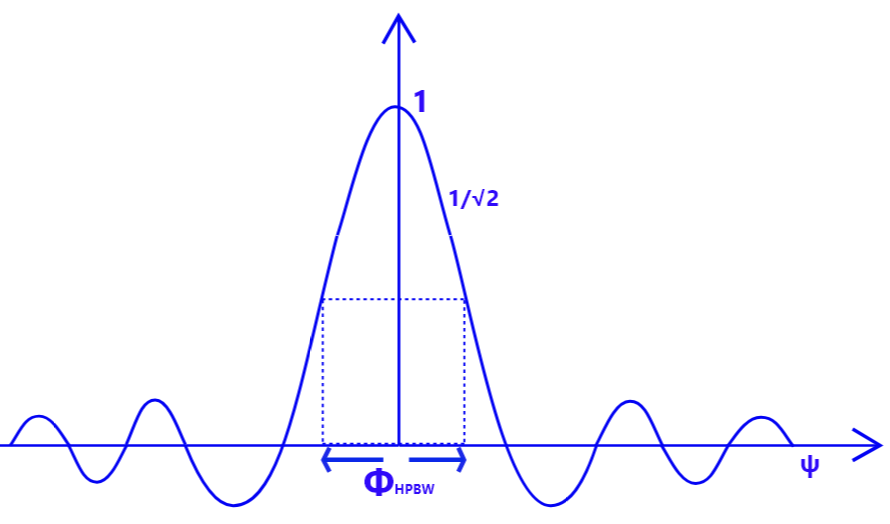
\includegraphics[width=1\linewidth]{fig54_1}
	\caption{}
	\label{54.1}
	
\end{figure}

Therefore from the radiation pattern given as:
$$
\frac{1}{N} \frac{\sin{(\frac{N \psi}{2})}}{\sin{(\frac{ \psi}{2})}}
$$
We equate it to $1/\sqrt{2}$ to get the angle $\psi$ corresponding to the $3dB$ points, given as:
\begin{equation}
\arrowvert \frac{1}{N} \frac{\sin{(\frac{N \psi}{2})}}{\sin{(\frac{ \psi}{2})}} \arrowvert = 1/\sqrt{2}
\end{equation}

However, the above problem cannot be solved analytically but it can be solved numerically, which is tedious. So instead, we will make an approximation. It is easier to find the angles $\psi$ for the first nulls than it is to find the angles $\psi$ for the $3dB$ points. So for large $N$ element arrays, we can approximate the radiation pattern between the first nulls as a straight line and so the half power beam width $\phi_{HPBW}$ can be approximated as half of the beam width between first nulls, that is:
\begin{equation}
\phi_{HPBW} \approx \frac{BWFN (\phi_{FN})}{2}
\end{equation}

Therefore, given a radiation pattern, all we need to do is find the first nulls and then find the beam width between first nulls $\phi_{FN}$, however, it should be kept in mind that depending upon the direction of maximum radiation, two nulls may not always be visible. Consider two radiation patterns shown in Figure \ref{54.2}. For the visible region where the direction of maximum radiation $\phi_{max}$ is given in some direction. Since the radiation pattern is a figure of revolution around the axis of the arrays, the same pattern is replicated as shown.

\begin{figure}
	\centering
	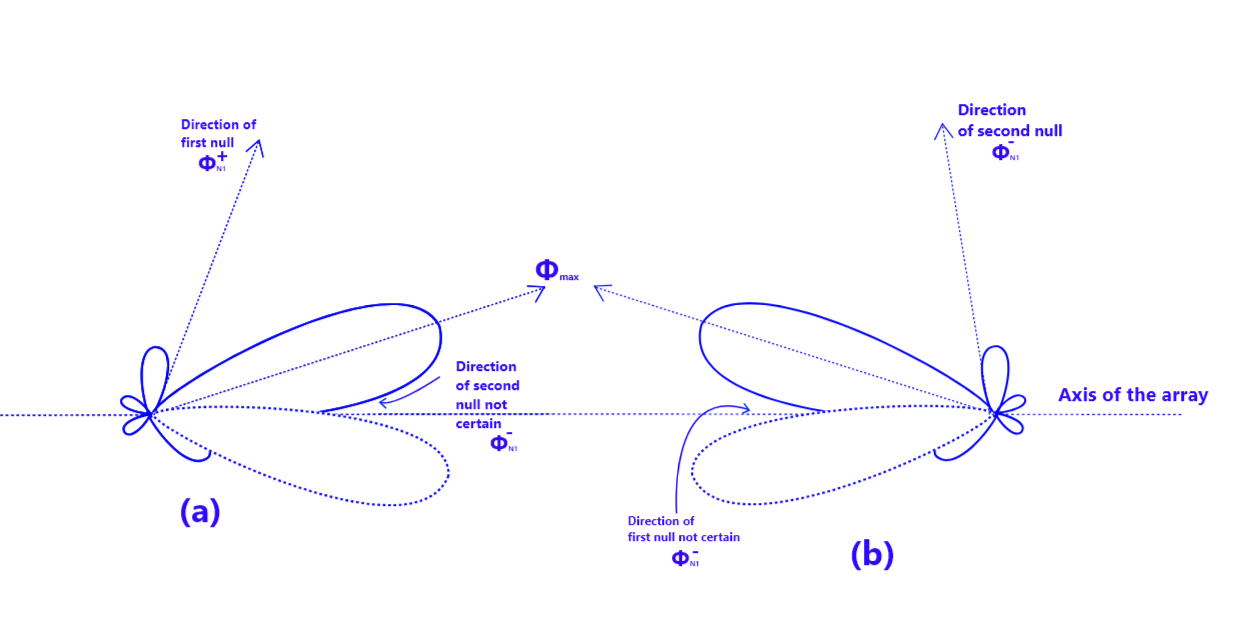
\includegraphics[width=1\linewidth]{fig54_2}
	\caption{}
	
	\label{54.2}
	
\end{figure}

It can be seen that for Figure \ref{54.2}a, the first null to the left of the maximum direction  is visible while the first null to the right of the maximum direction is not visible and then for Figure \ref{54.2}b, the reverse is the case. So if we rewrite the equation for finding the nulls which is:
\begin{equation}
\cos{\phi_{SL}} = \cos{\phi_{max}} \pm \frac{m \lambda}{N d} 
\end{equation}

For Figure \ref{54.2}a, it can be said that the null corresponding to the first null to the left is $\cos{\phi^+_{N_1}} = \cos{\phi_{max}} - \frac{ \lambda}{N d} $ and it falls within the range of $\cos{\phi_{SL}}$ which is $-1$ to $+1$, while the first null to the right is given by $\cos{\phi^-_{N_1}} = \cos{\phi_{max}} + \frac{ \lambda}{N d} $ and it does not fall within the range if $-1$ to $+1$. Similarly, the same can be said for Figure \ref{54.2}b only now in reverse. Therefore, this poses a problem to our approximation which is $\phi_{HPBW} = \frac{ \phi_{BWFN}}{2}$ so to solve this problem, we make further approximation and assume the nulls are equally spaced in the $\phi$  domain, therefore, the difference between any of the direction of the first nulls and the direction of the maximum radiation is approximately equal to the half power beam width of the array. We can best understand it this way. If we assume the nulls are equally spaced, then the expression:
$
\phi_{HPBW} \approx \frac{\phi^+_{N_1} - \phi^-_{N_1}}{2}
$
is half of the beam width between the first nulls which is equal to $\phi^+_{N_1} - \phi_{max}$ or  $\phi_{max} - \phi^-_{N_1}$.

So:
\begin{equation}
\begin{split}
\phi_{HPBW} & = \phi_{1}  - \phi_{2}\quad \text{from fig. \ref{54.3}}\\
&\approx \frac{\phi^+_{N_1} - \phi^-_{N_1}}{2} \\
& \approx \phi^+_{N_1} - \phi_{max} \\
& \approx \phi_{max} - \phi^-_{N_1}
\end{split}
\end{equation}

\begin{figure}
	\centering
	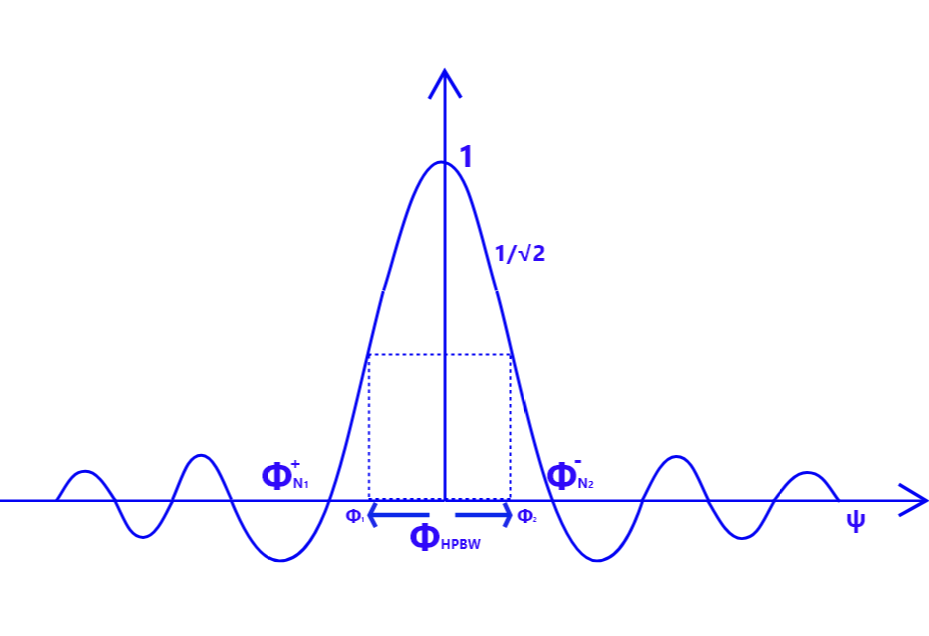
\includegraphics[width=1\linewidth]{fig54_3}
	\caption{}
	
	\label{54.3}
	
\end{figure}

With the approximation lets consider one of the cases where we know the $\phi_{N_1}^{+}$ and $\phi_{max}$, so $\phi_{HPBW} \approx \phi_{N_1}^{+} - \phi_{max} $ \\ 
We have $cos\phi_{N_1}^{+} = cos\phi_{max} - \dfrac{\lambda}{dN}$ which we rewrite as $cos\phi_{N_1}^{+} - cos\phi_{max} = - \dfrac{\lambda}{dN}$ \\ \\
Using the trig identities $cos(A - B) -cos(A + B) = 2sinAsinB$ \\ 
then $A - B = \phi_{N_1}^{+}$ and  $A + B = \phi_{max}$ \\ 
So, $ A = \dfrac{\phi_{N_1}^{+} + \phi_{max}}{2}$ and $B =  \dfrac{\phi_{max} - \phi_{N_1}^{+}}{2} $
$$cos\phi_{N_1}^{+} - cos\phi_{max} = 2sin (\dfrac{\phi_{N_1}^{+} + \phi_{max}}{2}) sin(\dfrac{\phi_{max} - \phi_{N_1}^{+}}{2})$$
$$ \Rightarrow  -2sin (\dfrac{\phi_{N_1}^{+} + \phi_{max}}{2}) sin(\dfrac{\phi_{N_1}^{+} - \phi_{max}}{2}) = - \dfrac{\lambda}{dN}$$ 
$$ \Rightarrow  2sin (\dfrac{\phi_{N_1}^{+} + \phi_{max}}{2}) sin(\dfrac{\phi_{N_1}^{+} - \phi_{max}}{2}) =  \dfrac{\lambda}{dN}$$
$\phi_{HPBW} \approx \phi_{N_1}^{+} - \phi_{max} $ and $\phi_{N_1}^{+} \approx \phi_{HPBW} + \phi_{max}$ \\
So, $2sin(\dfrac{\phi_{HPBW}}{2})sin(\dfrac{\phi_{max} + \phi_{HPBW}}{2}) = \dfrac{\lambda}{dN}$ \\ \\
Using trig identities, $sin(A+B) = sinAcosB + sinBcosA $ 
$$ 2sin(\dfrac{\phi_{HPBW}}{2})(sin\phi_{max}cos(\dfrac{\phi_{HPBW}}{2}) + sin(\dfrac{\phi_{HPBW}}{2})cos\phi_{max}) = \dfrac{\lambda}{dN} $$
Now if $N$ is very large ($N \gg 1$), the half power beam width is much smaller than $1$ ($\phi_{HPBW} \ll 1$) because the width between the first nulls is going to be very small. \\
Then we can make another approximation provided this condition is satisfied which is if  $x\ll1$ then $sinx \approx x$ and $cos x \approx 1$. \\ \\
Therefore, we have 
\begin{equation}
2\left(\dfrac{\phi_{HPBW}}{2}\right)\left(sin\phi_{max} + cos\phi_{max}\dfrac{\phi_{HPBW}}{2}\right) = \dfrac{\lambda}{dN}$$ 
$$ \phi^2_{HPBW}cos\phi_{max} + 2sin\phi_{max}\phi_{HPBW} = \dfrac{\lambda}{dN}
\label{eqn37}
\end{equation}
The approximate value of $\phi_{HPBW}$ can be obtained by solving the quadratic equation \ref{eqn37} as;
$$ \phi_{HPBW} = \dfrac{-2sin\phi_{max}\pm\sqrt{4sin^2\phi_{max} + \frac{4\lambda}{dN}cos\phi_{max}}}{2cos\phi_{max}}$$
$$ = \dfrac{-sin\phi_{max}\pm\sqrt{sin^2\phi_{max} + \frac{\lambda}{dN}cos\phi_{max}}}{cos\phi_{max}} $$
The equation above shows that as $\phi_{max}$ increase from $0$ to $\frac{\pi}{2}$, the beam width $\phi_{HPBW}$ decreases. That is when $\phi_{max} = 0$ (end-fire array) the HPBW is maximum and when $\phi_{max} = \frac{\pi}{2}$(broadside array) the HPBW  is minimum. Using equation \ref{eqn37}, we can get the HPBW for the two special antenna cases. \\ \\
For the broadside array ($\phi_{max} = \dfrac{\pi}{2}$), the HPBW is; 
$$ \phi^2_{HPBW}(0) + 2\phi_{HPBW} = \dfrac{2\lambda}{dN}$$
\begin{equation}
So, \ \phi_{HPBW} \approx \dfrac{\lambda}{dN}
\label{eqn39} 
\end{equation} 
For the end-fire array ($\phi_{max} = 0$), the HPBW is 
$$ \phi^2_{HPBW} + 2(0)\phi_{HPBW} = \dfrac{2\lambda}{dN} $$
\begin{equation}
So, \ \phi_{HPBW} \approx \sqrt{\dfrac{2\lambda}{dN}}
\label{eqn40}
\end{equation}
For an N element array where the inter-element spacing is d, the length of the array is (N - 1)d which is approximately $Nd$ for large $N(N\gg 1)$. So the equations for the two special cases can be written as: 
$$ \phi_{HPBW} \ for \ Broadside \ Array \approx \dfrac{\lambda}{length \ of \ array}$$ and
$$ \phi_{HPBW} \ for \ the \ end-fire \ array \approx \sqrt{\dfrac{2\lambda}{length \ of \  the \ array}}$$
It is seen that the half power beam width is inversely proportional to the length of the array in the broadside array whereas, it is inversely proportional to the square-root of the length of the array for the end-fire array. We therefore, conclude that for a given length the broadside array has much smaller HPBW compared to that of the end-fire array. Alternatively,
%PAGE 6/10
it can be said that the half power beam width $\phi_{HPBW}$ increases as we move from the broadside array to the end-fire array. This concept is applied in phased (scanning) array antenna. This array antenna is used to scan by electronically changing the phase and as the direction changes (while it is scanning ) the beam width changes.

\begin{figure}[h!]
	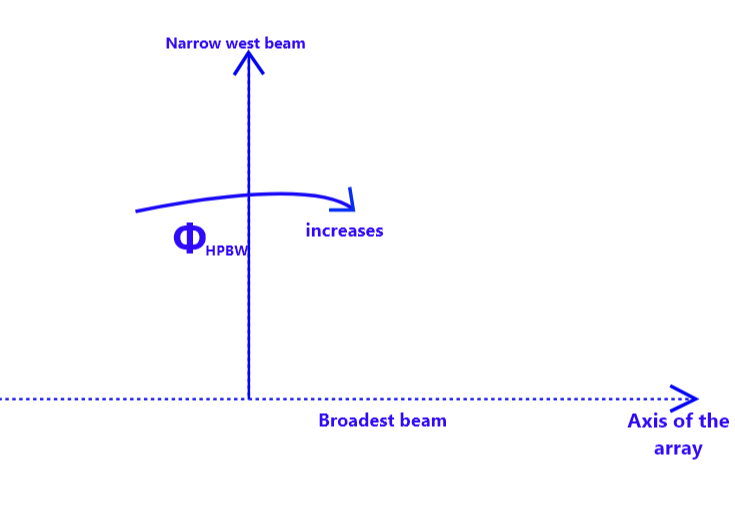
\includegraphics[width=1\linewidth]{fig54_4}
	\centering
	\caption{}
	
	\label{54.7}
	
\end{figure}

So changing the phase shift, not only changes the direction of the beam but also changes the beam width. 


\section{Directivity of Uniform Array}

As mentioned earlier, the directivity of an antenna defines its power focusing capability. Once the radiation pattern of an antenna is known, it's directivity can be calculated using equation \ref{eqn14b}.\\

For an N-element uniform array therefore the directivity is given by;
\begin{equation}
D = \frac{4 \pi}{\iint \arrowvert AF \arrowvert^2 d \Omega}
\label{eqn43}
\end{equation}


Where $AF$ is the normalized radiation pattern of the array and it is given as:
$$
\left\vert \frac{1}{N} \frac{\sin{(\frac{N \psi}{2})}}{\sin{(\frac{ \psi}{2})}} \right\vert
$$

Obviously, for a general uniform array, the equation of directivity \ref{eqn43} has to be evaluated numerically. For a large array however, one can make appropriate approximations to the integral $\iint \arrowvert AF \arrowvert^2 d \Omega$. The integral can be replaced by the solid angle within the half power beam width of the array. To get a better insight. Let us find the directivity of an $N$ element array in the broadside and the end-fire mode.

Figure \ref{54.8} shows the main beam of the array in three dimensional space. It is apparent that although the planar radiation pattern looks similar to the broadside and the end fire arrays, in three dimension, they have totally different appearance.The three dimensional main beam pattern for a broadside array looks like a disk, whereas for the end fire array, it appears like an elongated balloon.

\begin{figure}[h!]
	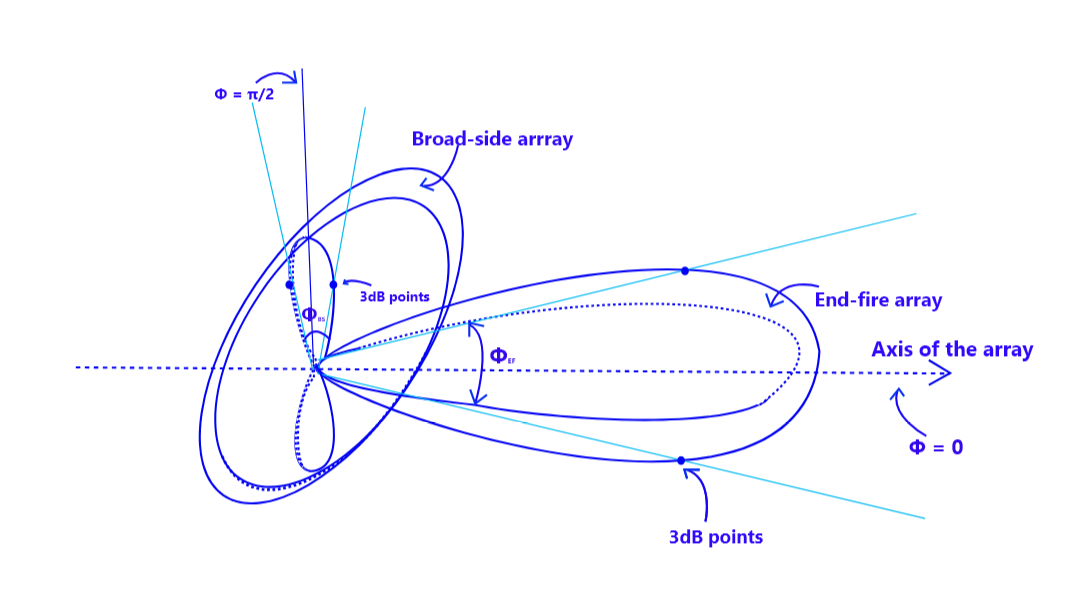
\includegraphics[width=1\linewidth]{fig54_5}
	\centering
	\caption{}
	
	\label{54.8}
	
\end{figure}

If we denote the $HPBW$ of the broadside and the end-fire array respectively by $\phi_{BS}$ and $\phi_{EF}$, from equations \ref{eqn39} and \ref{eqn40}, we get:

$$
\phi_{BS} = \frac{\lambda}{dN}
$$

$$
\phi_{EF} = \sqrt{\frac{2 \lambda}{dN}}
$$

The solid angle for the broadside array is approximately:

$$
\Omega_{BS} \approx 2 \pi \phi_{BS}
$$

Similarly, the solid angle for the end-fire array is approximately

$$
\Omega_{EF} \approx  \pi (\frac{\phi_{EF}}{2})^2
$$

Since the volume of the half power beam width approximates to a thin slab of thickness $\phi_{BS}$, length $2\pi$ and height of $1$ unit for the broadside array and for the end-fire array, it approximates to a cylinder of diameter $\phi_{EF}$ whose height is $1$ unit.

So the directivity,
$$
D \approx \frac{4 \pi}{\Omega}
$$

For the broadside array it is given as:

\begin{equation}
D_{BS} \approx \frac{4 \pi}{2\pi\phi_{BS}} \approx \frac{2dN}{\lambda}
\end{equation}
For the end-fire array, it is given as:

\begin{equation}
D_{EF} \approx \frac{4 \pi}{\pi (\frac{\phi_{EF}}{2})^2} \approx \frac{8dN}{\lambda}
\end{equation}

It should be noted that although the beam width of the broadside
is smaller than that of the end five array, the directivity of the end five array is higher by a factor of $4$. \\ \\
Lets consider an example below;
\begin{exmp}
	A two element array consists of collinear hertz dipole. The elements spacing is $\lambda/2$. Find the directivity of the array when the elements are excited in phase. 
\end{exmp}
\underline{\centering Solution} \\ 
Since the antenna element is the Hertz dipole, the primary element radiation is $\sin\theta$ 
\paragraph*{} The radiation patten of the array is \\ \\
= Primary radiation pattern $\times$ Array factor \\ \\
\begin{equation*}
= sin\theta \times \left|\dfrac{1}{N} \dfrac{sin(\frac{N \psi}{2})}{sin(\frac{\psi}{2})}\right|
\end{equation*}

since $N = 2$ \\
$$ = sin\theta \times \dfrac{1}{2} \dfrac{sin( \psi)}{sin(\frac{\psi}{2})} = \dfrac{1}{2} \dfrac{sin(\frac{\psi}{2}+ \frac{\psi}{2})}{sin(\frac{\psi}{2})} \times sin\theta $$ 
From Trig Identities $sin(\frac{\psi}{2}+ \frac{\psi}{2}) = 2sin\frac{\psi}{2}cos\frac{\psi}{2}$
$$ |E_{n}| = \dfrac{1}{2} \times \dfrac{2sin\frac{\psi}{2}cos\frac{\psi}{2}}{sin\frac{\psi}{2}}  \times sin\theta = sin\theta cos\frac{\psi}{2}	$$
$\psi = \beta dcos\theta +  \delta $ \\ \\
where, $\delta = 0$(in phase), $\beta = \frac{2\pi}{\lambda}$ and $ d = \frac{\lambda}{2} $ \\ \\
So $\psi = \frac{2\pi}{\lambda} \cdot \frac{\lambda}{2} cos\theta  = \pi cos\theta$ \\ \\
Therefore, $$|E_{n}| = sin\theta cos\left(\dfrac{\pi cos\theta}{2}\right) $$ 
Directivity: $ D = \dfrac{4\pi}{\int_{4\pi}|E_{n}(\theta, \phi)|^2 dA}$ 
$$ D = \dfrac{4\pi}{\int_{0}^{2\pi}\int_{0}^{\pi} sin^2\theta cos^2\left(\dfrac{\pi cos\theta}{2}\right)sin\theta d\theta d\phi}$$  $$ = \dfrac{4\pi}{ 2\pi \int_{0}^{\pi} sin^3\theta cos^2\left(\dfrac{\pi cos\theta}{2}\right) d\theta} = \dfrac{2}{I}$$
$ I = \int_{0}^{\pi} sin^3\theta cos^2\left(\dfrac{\pi cos\theta}{2}\right) d\theta $, 
let $t = \dfrac{\pi cos\theta}{2} $; $ cos\theta = \dfrac{2t}{\pi}$ \\ \\
$\dfrac{dt}{d\theta} = \dfrac{- \pi}{2} sin\theta $ ; $sin\theta d\theta = \dfrac{-2}{\pi}dt$, substituting\\ \\ we have
$$  I = \int_{0}^{\pi} sin^2\theta cos^2t\left(\dfrac{-2}{\pi}dt\right) $$
$$ = \int_{0}^{\pi} 1 - cos^2\theta \left(\dfrac{-2 cos^2 t}{\pi} dt\right) $$ 
$$  = \int_{0}^{\pi} 1 - \dfrac{4t^2}{\pi^2} \left(\dfrac{-2 cos^2 t}{\pi} dt\right)$$
Changing the limits
$$  = \int_{\frac{\pi}{2}}^{-\frac{\pi}{2}} -\dfrac{2}{\pi}\left(1 - \dfrac{4t^2}{\pi^2}\right) cos^2t dt$$
$$  = \int_{-\frac{\pi}{2}}^{\frac{\pi}{2}} \dfrac{2}{\pi}\left(1 - \dfrac{4t^2}{\pi^2}\right) cos^2t dt$$
$$ I = 0.8677 $$ 
The directivity of the array  is; 
$$ D = \dfrac{2}{0.8677} = 2.3 $$ 
\section{GRATING LOBES}
As mentioned earlier when $\psi = 0 $ or multiples of $2\pi$, there is a maximum. Recall that the direction of maximum for an array is chosen at $\psi = 0$ so that it is symmetric along the range of $\psi$. However, at every multiple of $2\pi$ there will be a maximum as shown in Figure \ref{54.9} and these maximums are called grating lobes. So a grating lobe or grating beam is a beam identical to the main beam but in an undesired direction. The presence of grating lobes causes the power radiated by the array to get divided between the main beam and these lobes and therefore the power efficiency in the direction of the main beam is consequently reduced. The grating lobes are normally avoided in the radiation pattern.

\begin{figure}[h!]
	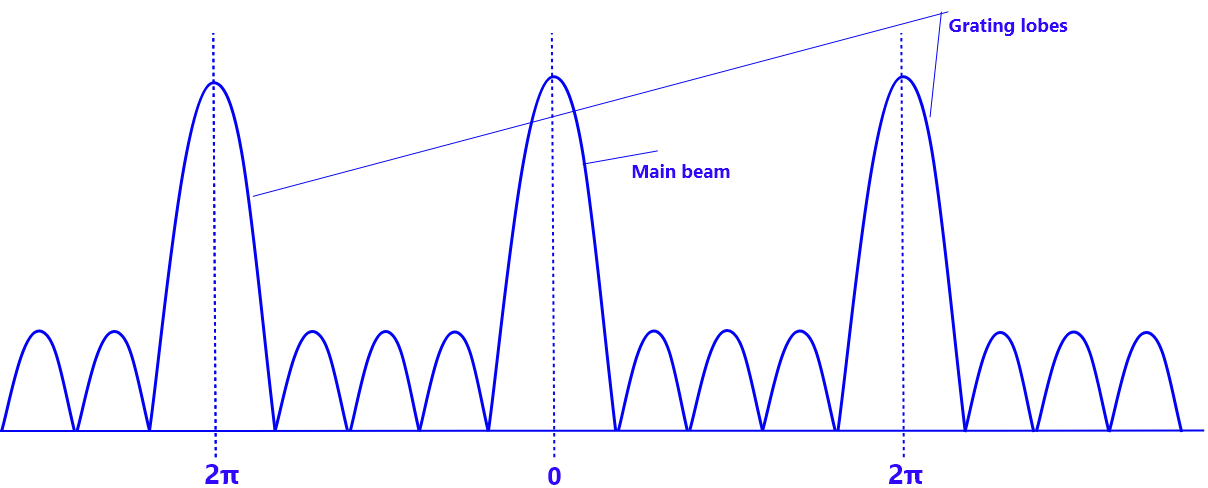
\includegraphics[width=1\linewidth]{fig54_6}
	\centering
	\caption{}
	\label{54.9}
	
\end{figure}

For the broad side array $(\phi_{max} = \pi/2)$ and the visible range of $\psi$ is between $-Bd$ and $+Bd$, that is
$$
-Bd \leq \psi_{visible} \leq Bd \quad \text{which is symmetric at $\psi =0$}
$$
Therefore, to avoid grating lobes, $Bd$ should be less than $2\pi$. That is for the broadside array, if $Bd < 2\pi$, there would be no grating lobes. Substituting for $\beta = \frac{2\pi}{\lambda}$, we get condition for no grating lobe of a broadside array as:
$$d < \lambda $$

Also for the end-fire array, assuming the main beam is also along $\phi_{max} = 0$, the visible range of $\psi$ is:
$$
0 \leq \psi_{visible} \leq 2Bd \quad \text{such that $\psi_{max}$ symmetric along the range}
$$

To avoid grating lobes in this case, $2Bd < 2 \pi$ and so $d < \lambda/2$. There is no grating lobe irrespective of the direction of the main beam. In practice therefore, all the scanning beam phased array have inter-element spacing of $\lambda /2$. Note that to avoid grating lobes strictly, the inter-element spacing should be less than $\lambda / 2$ but in practice, the scanning range of the main beam is a little short of $0$ to $\pi$ and therefore $d=\lambda/2$ is used without getting any grating lobes.

Before closing the discussion on grating lobes, it should be mentioned that grating lobes can be suppressed by properly choosing the primary radiation pattern of the array elements. With  non-isotropic array elements, it is possible to increase the inter-element spacing beyond $\lambda/2$ without encountering the grating lobes.